\section{Approach} \label{sec:Approach}

%%%%%%%%%%%%%%%%%%%%%%%%%%%%%%%%%%%%%%%%%%%%%%%%%%%%%%%%%%%%%%%%%%%%%%%%%%%
%% Discuss:
%%     your approach to the problem
%%   
%%     why its good or better
%%   
%%     details of solution (no results)
%%   
%%     where did your data come from
%%   
%%     where did your model(s) come from
%%   
%%     algorithms to be used
%%   
%%     how will you explore the parameter space
%% 
%%     analysis to be done on data
%% 
%%%%%%%%%%%%%%%%%%%%%%%%%%%%%%%%%%%%%%%%%%%%%%%%%%%%%%%%%%%%%%%%%%%%%%%%%%%
In this section we will first present reasons \emph{why} the afforementioned
programming methods will not work well, followed by motivation to use the
methods we did. After these rather nebulous postulations, we will discuss
\emph{our} particular implementation, starting from the ground up. Finally
we will explain what data we collected and why we believed they were important.

\subsection{Ineffective Theory}

\subsubsection{Traditional Procedural Programming}
Consider a stream or river. (Disclaimer: this is a massive simplification of
one of natures most majestic features.) Despite potentially massive deluges, 
the model is still fairly predictible: water starts at the source and flows 
down to the mouth. If we use the analogy of the water in a river being data 
flow in a program, we can say that if the water reaches the river delta, it
has sucessfully arrived at its goal.

But what of lakes and seas? There is still current in the water, but when
can one say that it has reached its ``goal?'' Where did it start in the first
place?

Likewise, when has our agent reached its goal? Perhaps we could say it is 
when the agent has consumed all the food in Flatworld, but was the agent 
efficient in doing so? Let us consider the potential program flow that
would be required for modelling an agent's simple decision whether to eat one
object it sees compared with another:

\begin{verbatim}
  if object0 is food
    if object0 is only object in sight
      eat object0
    else if object1 is food
      if object1 is closer than object0
        eat object1 
      else
        eat object0
  rinse and repeat
\end{verbatim}

This could be rearranged in multiple ways to produce the same behavior,
but the result would be the same; even this simple action is quite cumbersome
to implement.

\subsubsection{Declarative (e.g. Logic) Programming}
Say we look at this same decision and action from a declarative programming
paradigm, and specifically implementing first order predicate logic.
\begin{equation} \label{eq:logic1}
  \large
  \begin{aligned}
    \exists\ obj_i \in &\{Food\ \wedge\ \forall obj_n \in Food, \text{where }
    n \neq i, \neg closer(obj_n,obj_i)\}
  \end{aligned}
\end{equation}

Equation \eqref{eq:logic1}, like the code above, describes whether or 
not to eat an object. If \eqref{eq:logic1} evaluates as $True$, then the agent 
will be told to eat the object. Now we have introduced other problems! For 
instance, we have the set $Food$ to initially populate \emph{and} parse 
through every time the agent considers an object. 

\subsubsection{As if it Wasn't Bad Enough Already...}
These two approaches have already proven to be ineffective in accomplishing
our goal, but then we must enforce a particularly harsh constraint: 
\textbf{there is no oracle in Flatworld}. That is, the agent must acquire
important knowledge on its own. Object distance and type are not simply
dictated to the agent.\footnote{Although later we shall reveal that we did
do this, and discuss why we could justify this.} Even though creating and
scanning the set $Food$ can be done in $O(n)$ time, our agent has no working
knowledge of where all the food objects are, or even how many exist
in Flatworld.


\subsection{Effective Theory}
It may not come as a surprise that we decided to approach this problem using
neural networks. We were perhaps a little harsh on our discussion of 
procedural programming. First of all, Flatland itself is implemented in C,
along with the agent. Secondly, we can still apply the mathematics involved
in neural networks with procedural languages like C. Rather than using a
rigid conditional structure, however, we programmed our agent's brains to
be able to adjust themselves based upon the situations the agent encounters.

\subsection{Our Implementation}
{\Large NEA: AM I COVERING ALL THE BASES?}
For all of our runs we used a shim\footnote{See section~\ref{sec:Ack}.} that 
sat between the original C code and our Python code. This served two purposes:
since we already had a functional object to describe neurons in Python we could
recycle it for this project; that and we only had to compile the C code once.
Given the number of minute changes we made to each incarnation of our brains,
avoiding recompiling every time allowed for immediate gratification (or 
disappointment) on our part.

 Our next goal was to create an agent who
would move blindly and devour any food/poison/placebo objects in its path.
As we improved its capabilities, the agent started to descriminate between 
helpful and detrimental objects, and ultimately it would only consume food 
objects when it was in need of food (i.e. it will not be a gluttonous agent).

\subsection{Brain Design}

\subsubsection{Brain 0}
We started from the most simplistic of models: an agent who sat in place until
it died. There is not much more to say about this model, other than it shunned
all of its inputs, and used none of its functions.

\begin{figure}
\begin{center}
  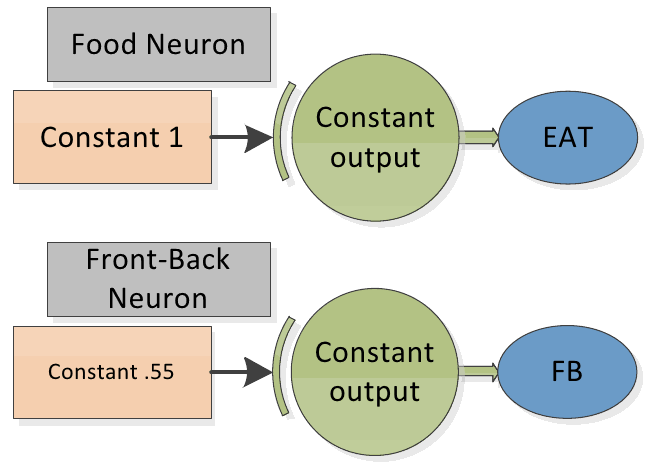
\includegraphics[scale=.3]{img/brain1.png}
  \caption{Active neurons in Brain 1}
  \label{fig:brain1}
\end{center}
\end{figure}

\subsubsection{Brain 1}

Our second brain (Fig. \ref{fig:brain1}) constantly activates the agent's 
eating actuator (i.e. the agent will try to eat anything with which it comes
in contact.

\subsubsection{Brain 2}

Brain 2 was the first neural network to take advantage of the agent's visual
cortex (Fig. \ref{fig:brain2}). Of the 31 eyelets available to the agent, it 
used only the data it received from it's center eyelet (eyelet 15).


\begin{figure}
\begin{center}
  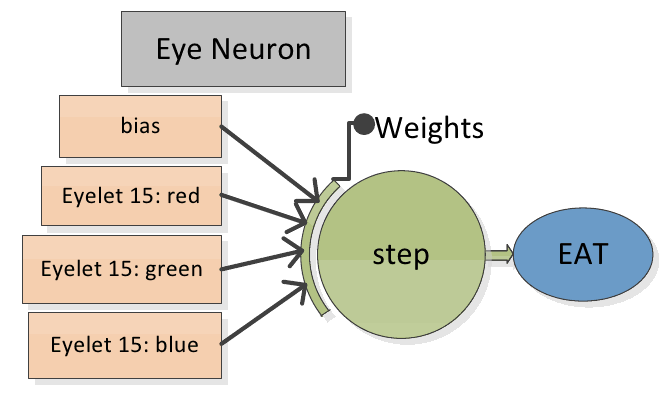
\includegraphics[scale=.3]{img/brain2.png}
  \caption{Brain 2's visual neuron}
  \label{fig:brain2}
\end{center}
\end{figure}
